\documentclass[11pt,a4paper]{ltxdoc} 
\usepackage[spanish,es-noindentfirst,es-tabla]{babel}

\usepackage[utf8]{inputenc}
\usepackage[T1]{fontenc}
\usepackage{graphicx}
\usepackage{xcolor}
\usepackage{float}
\usepackage[margin=2.5cm,left=3.5cm]{geometry}

\setlength{\parskip}{0.2\baselineskip}
\renewcommand{\baselinestretch}{1.1}

\newcommand{\file}[1]{\texttt{#1}}
\newcommand{\option}[1]{\texttt{#1}}
\newcommand{\package}[1]{\texttt{#1}}

\title{\file{aleph-notas.cls}}
\author{Proyecto Alephsub0\\ Andr\'es Merino}
\date{2022-10-26\\ Versión 2.0.1b}

\usepackage[colorlinks,linkcolor=teal,urlcolor=teal,
   citecolor=black,bookmarks=true]{hyperref}
\usepackage{url}

\begin{document}
 
\maketitle
 
\begin{abstract}
    \file{aleph-notas.cls} es una clase creada para dar formato a notas y resúmenes, encaminadas a ser libros bajo la clase |aleph-libro.cls|. Esta clase genera el encabezado, los ambientes utilizados, entre otros. Esta clase fue generada dentro del proyecto Alephsub0 (\url{https://www.alephsub0.org/}).

    \color{red}
    La actual documentación corresponde a versión 2.0.1b (beta) que incluye algunas novedades. 
    \begin{enumerate}
        \item Se elimina el formato clásico para el estilo de los teoremas.
        \item Se añade la posibilidad de seleccionar fuentes: Palatino Linotype (mathpaso) y Monstserrat
    \end{enumerate}
\end{abstract}

\section{Introducción}

La clase \file{aleph-notas.cls} es parte del conjunto de clases y paquetes creados por Andrés Merino dentro de su proyecto personal Alephsub0. Está basada en la clase \file{pubciencias-libro.cls} que recoge el formato de los primeros libros editados en la Unidad de Publicaciones de la EPN.

\section{Uso}

Para cargar la clase se utiliza: \cs{documentclass}\oarg{opciones}|{aleph-notas}| con las opciones acordes al formato que se desee.

Para visualizar un ejemplo puedes acceder al repositorio de GitHub de esta clase (clic \href{https://github.com/mate-andres/LaTeX_aleph-notas}{aquí}) % o buscarlo en la galería de plantilla de Overleaf (clic \href{https://www.overleaf.com/latex/templates/plantilla-para-escribir-resumenes-de-clase/mftfvjfhdcyj}{aquí}).


\subsection{Opciones}

Las opciones de la clase son las siguientes:
\begin{description}
    \item[|10pt|, |11pt|, |12pt|] ajustan el tamaño de fuente. Por defecto, se usa |10pt|.
    \item[|amplio|, |compacto|, |a4|, |a5|] genera la geometría de las notas predeterminada, es decir, tamaño de página y márgenes. Las dimensiones generadas por por estas opciones están dadas en la Tabla~\ref{tab:01}. Por defecto, se usa |compacto|.
    \item[|comentarios|, |codigo|] muestran el contenido de los ambientes opcionales |comentario| y |código|. Por defecto, no se muestra el contenido de estos ambientes.
\end{description}
  
\begin{table}[ht]
    \centering
    \begin{tabular}{cccccc}\hline
        Opción & Dimensiones & Interno & Externo & Superior & Inferior \\\hline
        |amplio| & 195mm$\times$265mm & 2.2cm & 2.2cm & 2.25cm & 2.25cm\\
        |compacto| & 160mm$\times$240mm & 1.7cm & 1.7cm & 2cm & 2cm\\
        |a4| & A4 & 2.2cm & 2.2cm & 2.25cm & 2.25cm\\
        |a5| & A5 & 2.2cm & 1cm & 2.25cm & 2.25cm\\
        \hline
    \end{tabular}
    \caption{Geometría de página predefinida.}
    \label{tab:01}
\end{table}

\subsection{Colores}

Las clase trabaja con un color básico:
\begin{description}
    \item[|colordef|] es el color preestablecido para los ambientes de teoremas y notas al margen. El color predefinido por la clase es $(0.81,0.62,0.00,0.22)$ del formato |cmyk|.
    \item[|colortext|] es el color preestablecido para los títulos $(0.81,0.62,0.00,0.22)$ del formato |cmyk|.
\end{description}
Se puede cambiar fácilmente estos colores con el comando\\
    \hspace*{3em}\cs{definecolor}|{colordef}|\marg{formato de color}\marg{color}\\
    \hspace*{3em}\cs{definecolor}|{colortext}|\marg{formato de color}\marg{color}

\section{Comando para tipografía}

Para esta nueva versión se incluye el comando \verb|\fuente|

\DescribeMacro{\fuente} 
    El comando fuente tiene el formato\\
        \hspace*{3em}\cs{fuente}\marg{nombre fuente},\\
    el \meta{nnombre fuente} especifica el tipo de paquete de fuente incluido en el documento, las opciones son: mathpazo y monstserrat.

\subsection{Comandos de datos informativos para las notas}

\DescribeMacro{\autor} 
    El comando autor tiene el formato\\
        \hspace*{3em}\cs{autor}\oarg{nombre de autor corto}\marg{nombre autor},\\
    el \meta{nombre de autor corto} se utiliza en el encabezado, mientras que \meta{nombre autor} se utiliza en el resto de lugares necesarios. De no especificarse el \meta{nombre de autor corto}, ambas variables son iguales.

\DescribeMacro{\institucion} 
    El comando institucion tiene el formato\\
        \hspace*{3em}\cs{institucion}\marg{nombre de la institución}.\\
    este comando es obligatorio.

\DescribeMacro{\carrera} 
\DescribeMacro{\asignatura}
\DescribeMacro{\fecha} 
    Los comandos \cmd{\carrera}, \cmd{\asignatura} y \cmd{\fecha} dan la información que se utilizará en el encabezado, todas estas son obligatorias para generar exámenes u hojas de datos. No son empleadas al generar hojas de respuestas. % El contenido de \cmd{\materia} y \cmd{\nota} se despliega en forma centrada mientras que el de \cmd{\autor} y \cmd{\fecha} se despliega en los extremos de la página.

\DescribeMacro{\tema}
    El comando \cmd{\tema} agrega información para el encabezado pero es opcional.
    
\DescribeMacro{\logouno}
\DescribeMacro{\logodos}
    Los comandos \cmd{\logouno} y \cmd{\logodos} definen el archivo de logo a ser utilizado, ninguno de los dos es obligatorio.  Cada comando tiene un argumento opcional en el cual se puede especificar el tamaño del logo, el predefinido es de 0.1 longitud de linea.
    
\subsection{Comandos varios}

\DescribeMacro{\encabezado}
    El comando \cmd{\encabezado} genera el encabezado de la página, no tiene ninguna opción.

\newpage
\subsection{Estilo de teoremas}

\DescribeEnv{ejem}
\DescribeEnv{obs}
\DescribeEnv{prop}
\DescribeEnv{cor}
\DescribeEnv{lem}
\DescribeEnv{teo}
\DescribeEnv{defi}
\DescribeEnv{axioma}
\DescribeEnv{ejer}
    Existen dos estilos de teoremas definidos: recuadro sin título aparte y recuadro con título aparte. Los ambientes predefinidos son: 
\begin{description}
    \item[|ejem|] para ejemplos, no utiliza recuadro, se numeran según la sección.
    \item[|obs|] para observaciones, no utiliza recuadro, por defecto no se numera a menos que se tenga la opción |numobs|.
    \item[|prop|{,} |cor|{,} |lem|] para proposiciones, corolarios y lemas, utiliza recuadro sin título aparte. Se numeran según la sección.
    \item[|teo|] para teoremas, utiliza recuadro con título aparte izquierdo. Se numeran continuando |prop|.
    \item[|defi|] para definiciones, utiliza recuadro con título aparte izquierdo. Se numeran según la sección.
    \item[|axioma|] para axiomas, utiliza recuadro con título aparte izquierdo. Se numeran según el sección.
    \item[|ejer|] para ejercicios, utiliza recuadro sin título aparte con la opción. Se numeran según el sección.
\end{description}

\subsection{Estilo de advertencia}

\DescribeEnv{advertencia}
    Este ambiente genera un recuadro amarillo sin título, pensado originalmente para colocar advertencias llamativas. Se pueden generar ambientes similares a este bajo la siguiente sintaxis:\\
    \hspace*{3em}\cs{newtcolorbox}\marg{nombre del ambiente}\verb"{postit}"
    

\subsection{Ambientes opcionales}

    Los ambientes descritos en esta sección están programados para que, dependiendo de las opciones de la clase, aparezcan o no al momento de compilar el documento. Esto es de utilidad si se quieren tener varias versiones del documento.

\DescribeEnv{codigo}
\DescribeEnv{comentarios}
    Los ambientes opcionales son |codigo| que se utiliza para poner código de programación, útil para manuales de laboratorio. Además, tenemos el ambiente |comentarios|, utilizado para agregar los comentarios destinados al docente.


\section{Ejemplos}

El inicio de un nota utilizando esta clase suele tener la siguiente forma:
\begin{verbatim}
    \documentclass[compacto,10pt]{aleph-notas}

    % -- Paquetes adicionales
    \usepackage{enumitem}
    \usepackage{aleph-comandos}
    
    % -- Datos de las notas
    \institucion{Proyecto Alephsub0}
    \autor{Andrés Merino}
    \carrera{Enfermería}
    \asignatura{Bioestadística}
    \autor{Mat. Andrés Merino}
    \tema{Cronograma y evaluaciones}
    \fecha{Semestre 2022-1}

    \logouno[0.25\textwidth]{Logos/logo02.eps}
    
    \definecolor{colordef}{cmyk}{0.81,0.62,0.00,0.22}
    \definecolor{colortext}{cmyk}{0.81,0.62,0.00,0.22}
    
    \begin{document}
    
    \encabezado
    
    \end{document}
\end{verbatim}
Con esto se obtiene las imágenes indicadas en la Figura~\ref{fig:01}.

\begin{figure}[h]
    \centering
    \fbox{\includegraphics[scale=0.5]{pag01.eps}}
    \caption{Ejemplo de notas}
    \label{fig:01}
\end{figure}

También se pueden generar más ambientes de teoremas, con otros formatos y colores, siguiendo los ejemplos que se muestran en el paquete \package{aleph-libro.cls} (\url{https://www.alephsub0.org/recursos/}).

\subsection{Problemas}

\begin{itemize}
\item 
    La versión actual trabaja bien en la versión de TeXLive 2019 en adelante (específicamente, con el paquete \package{tcolorcox} v4.20). Si se usa una versión anterior, existe una incompatibilidad con la actualización del paquete. Para utilizar versiones anteriores de ese paquete, es necesario cambiar:
    \begin{itemize}
        \item |tcbcolback| por |tcbcol@back|
        \item |tcbcolframe| por |tcbcol@frame|
    \end{itemize}
\end{itemize}

Cualquier problema adicional, por favor reportarlo a\\ 
\url{mat.andresmerino@gmail.com}.

\newpage
\DocInput{aleph-notas.dtx}

\end{document}
